\documentclass[12pt]{article}
\usepackage{amsmath, setspace}
\usepackage[margin=1in]{geometry}
\usepackage[linesnumbered,ruled]{algorithm2e}
\usepackage{graphicx}
\usepackage[english]{babel}
\usepackage{amsthm}
\usepackage{amssymb}
\usepackage{array}
\usepackage{subfigure}
\usepackage[latin1]{inputenc}
\usepackage{enumerate}
\usepackage{xspace}
\usepackage{amsfonts}
\usepackage{amsmath}
\usepackage{hyperref}
\usepackage{caption}
\usepackage{booktabs}
\usepackage{color}
\usepackage{lmodern}
\usepackage{tikz}
\usepackage{comment}
\usepackage{enumitem}
\usepackage{pgfplots}
\usepackage{lipsum}


\usetikzlibrary{shapes}
\usetikzlibrary{snakes}
\usetikzlibrary{backgrounds}
\usetikzlibrary{calc}


\newtheorem{thm}{Theorem}
\newtheorem{lem}{Lemma}
\newtheorem{rmk}{Remark}
\newtheorem{prop}{Proposition}
\newtheorem{dfn}{Definition}
\newtheorem{ex}{Example}
\newtheorem*{pf}{Proof}

\spacing{1.5}


% Natbib setup for author-year style
\usepackage{natbib}
 \bibpunct[, ]{(}{)}{,}{a}{}{,}%
 \def\bibfont{\small}%
 \def\bibsep{\smallskipamount}%
 \def\bibhang{24pt}%
 \def\newblock{\ }%
 \def\BIBand{and}%

\title{TITLE}
\author{} 
%%%%%%%%%%%%%%%%%%%%%%%%%%%%%%%%%%%%%
%%%%%%%%%% DON'T FORGET: NO AUTHORS %%%%%%%%%%
%%%%%%%%%%%%%%%%%%%%%%%%%%%%%%%%%%%%%
\date{}

\begin{document}
\maketitle
\begin{abstract}%

\lipsum[1]

\smallskip
\noindent \textbf{Keywords.} lorem; ipsum; dolor sit amet.

\end{abstract}%

\section{Introduction}

\lipsum[1]

\subsection{Outline}

\lipsum[2]

\subsection{Your subsections here}

\lipsum[3-5]

\subsubsection{A subsubsection}

\lipsum[6]

\paragraph{A paragraph.} \lipsum[7]

\section{Citations}

You can cite interesting work in lorem \citep{doe1999lorem} and lipsum \citep{doe2001lipsum}, or you can reference the authors immediately: \cite{madani2009loremipsum} fundamentally changed the field with their lorem ipsum {\em dolor sit amet} contribution.

\section{Figures, Tables, Algorithms}

For a visual example, please refer to Figure \ref{figExample1} and Figure \ref{figExample2}. Clearly, we see the following. \lipsum[1]

\begin{figure}[htbp]
\centering
\caption{You can use {\em tikz} or {\em PSTricks} to create your figures. \label{figExample1}}
 \resizebox{0.25\textwidth}{!}{
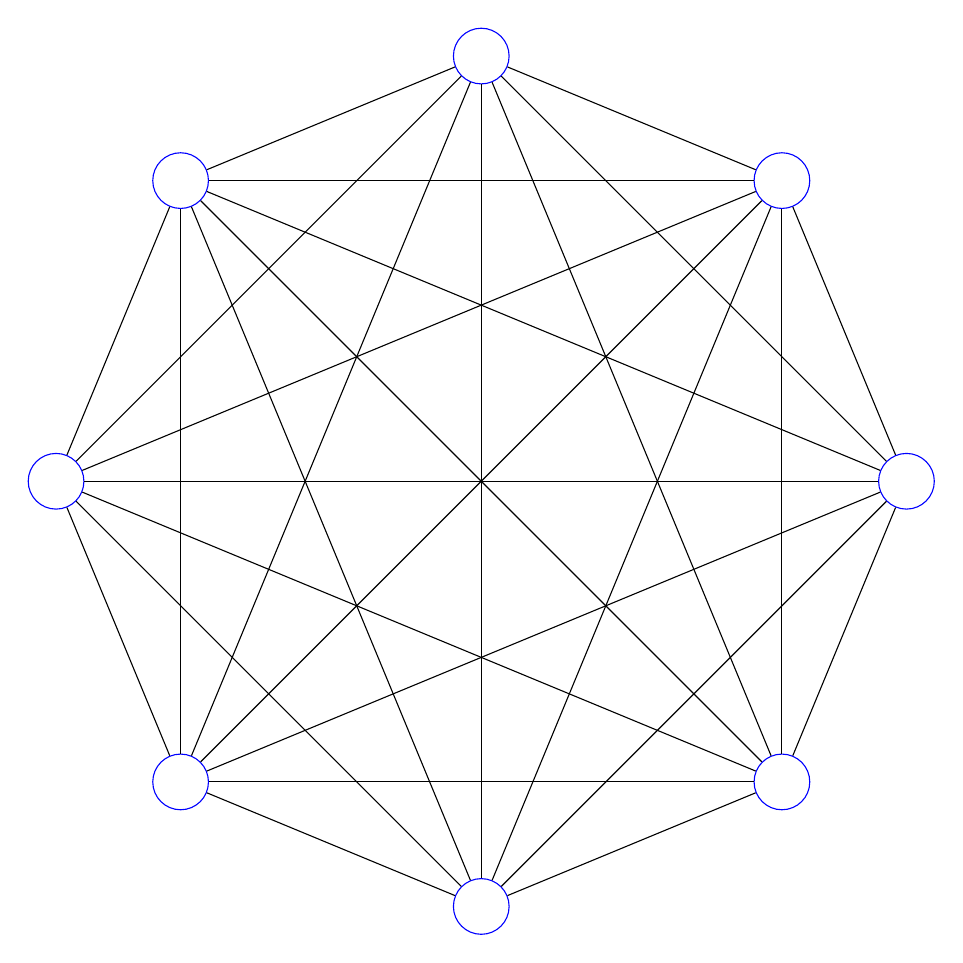
\begin{tikzpicture}[transform shape]
  \foreach \x in {1,...,8}{%
    \pgfmathparse{(\x-1)*45+floor(\x/9)*22.5}
    \node[draw,blue,circle,inner sep=0.25cm] (N-\x) at (\pgfmathresult:5.4cm) {};
  } 
  \foreach \x [count=\xi from 1] in {2,...,8}{%
    \foreach \y in {\x,...,8}{%
    \path (N-\xi) edge[-] (N-\y);
  }
}    
\end{tikzpicture}
 }
\end{figure}

\begin{figure}[htbp]
\centering
\caption{Or you can simply include them! \label{figExample2}}
 \includegraphics[scale=0.65]{example.pdf}
\end{figure}



To solve the problem, we devise Algorithm \ref{algExample}. It works as follows. \lipsum[2-4]

\begin{algorithm}[htbp]
    \caption{Random set of numbers. \label{algExample}}
    \SetKwInOut{Input}{Input}
    \SetKwInOut{Output}{Output}
    \underline{function RandomTesting} $(i, j, n)$\;
    \Input{Integer numbers $i, j, n$}
    \Output{The set of all divisors of $i$ and $j$ from 2 to $n$.}
    $S\leftarrow \emptyset$\;
     \For{$k\in \{2,\dots,n\}$}{
     	\If{$i\ \mathrm{mod}\ k$ and $j\ \mathrm{mod}\ k$}{
		$S\leftarrow S\cup\{k\}$\;
		}  	
  }
  	\Return $S$
\end{algorithm}

Our computational results on several instances are shown in Table \ref{tabExample}. \lipsum[5]

\begin{table}[htbp]
\centering
\caption{A Table. \label{tabExample}}
\begin{tabular}{l|rrrrrr}
Header 1 & Blah & Blah & Blah & Blah & Blah \\
\toprule
\emph{Instance 1} & 4,515 &  104,407  & 1,221.10 & 10 & 5 \\
\emph{Instance 2} &  1,234 &  13,345  & 345.67 & 20 & 5 \\
\emph{Instance 3} & 2,222 & 14,876  & 567.89 & 10 & 4 \\
\emph{Instance 4} & 4,123 & 35,234  & 567.98 & 30 & 5 \\
\emph{Instance 5} & 7,312  & 99,999  & 499.01 & 40 & 6 \\
\end{tabular}
\end{table}

\section{Concluding remarks}

Make sure to have all references to your identity, including acknowledgement of support, removed before final submission. Good luck!


\bibliographystyle{named} 
\bibliography{bibliography} 






\end{document}

